% Exam Template for UMTYMP and Math Department courses
%
% Using Philip Hirschhorn's exam.cls: http://www-math.mit.edu/~psh/#ExamCls
%
% run pdflatex on a finished exam at least three times to do the grading table on front page.
%
%%%%%%%%%%%%%%%%%%%%%%%%%%%%%%%%%%%%%%%%%%%%%%%%%%%%%%%%%%%%%%%%%%%%%%%%%%%%%%%%%%%%%%%%%%%%%%

% These lines can probably stay unchanged, although you can remove the last
% two packages if you're not making pictures with tikz.
\documentclass[11pt]{exam}
\RequirePackage{amssymb, amsfonts, amsmath, latexsym, verbatim, xspace, setspace}
\RequirePackage{tikz, pgflibraryplotmarks}

% By default LaTeX uses large margins.  This doesn't work well on exams; problems
% end up in the "middle" of the page, reducing the amount of space for students
% to work on them.
\usepackage[margin=1in]{geometry}
\usepackage{enumerate}
\usepackage{amsthm}

\theoremstyle{definition}
\newtheorem{soln}{Solution}

% Here's where you edit the Class, Exam, Date, etc.
\newcommand{\class}{Math 150A Section 8 and 16}
\newcommand{\term}{Spring 2020}
\newcommand{\examnum}{Practice Exam I Solutions}
\newcommand{\examdate}{February 13, 2020}
\newcommand{\timelimit}{1 hour 50 Minutes}

% For an exam, single spacing is most appropriate
\singlespacing
% \onehalfspacing
% \doublespacing

% For an exam, we generally want to turn off paragraph indentation
\parindent 0ex

\begin{document} 

% These commands set up the running header on the top of the exam pages
\pagestyle{head}
\firstpageheader{}{}{}
\runningheader{\class}{\examnum\ - Page \thepage\ of \numpages}{\examdate}
\runningheadrule

\begin{flushright}
\begin{tabular}{p{2.8in} r l}
\textbf{\class} & \textbf{Name (Print):} & \makebox[2in]{\hrulefill}\\
\textbf{\term} &&\\
\textbf{\examnum} & \textbf{Student ID:}&\makebox[2in]{\hrulefill}\\
\textbf{\examdate} &&\\
\textbf{Time Limit: \timelimit} % & Teaching Assistant & \makebox[2in]{\hrulefill}
\end{tabular}\\
\end{flushright}
\rule[1ex]{\textwidth}{.1pt}


This exam contains \numpages\ pages (including this cover page) and
\numquestions\ problems.  Check to see if any pages are missing.  Enter
all requested information on the top of this page, and put your initials
on the top of every page, in case the pages become separated.\\

You may \textit{not} use your books or notes on this exam.  However, you may use a \textit{basic} calculator.\\

You are required to show your work on each problem on this exam.  The following rules apply:\\

\begin{minipage}[t]{3.7in}
\vspace{0pt}
\begin{itemize}

%\item \textbf{If you use a ``fundamental theorem'' you must indicate this} and explain
%why the theorem may be applied.

\item \textbf{Organize your work}, in a reasonably neat and coherent way, in
the space provided. Work scattered all over the page without a clear ordering will 
receive very little credit.  

\item \textbf{Mysterious or unsupported answers will not receive full
credit}.  A correct answer, unsupported by calculations, explanation,
or algebraic work will receive no credit; an incorrect answer supported
by substantially correct calculations and explanations might still receive
partial credit.  This especially applies to limit calculations.

\item If you need more space, use the back of the pages; clearly indicate when you have done this.

\item \textbf{Box Your Answer} where appropriate, in order to clearly indicate what you consider the answer to the question to be.
\end{itemize}

Do not write in the table to the right.
\end{minipage}
\hfill
\begin{minipage}[t]{2.3in}
\vspace{0pt}
%\cellwidth{3em}
\gradetablestretch{2}
\vqword{Problem}
\addpoints % required here by exam.cls, even though questions haven't started yet.	
\gradetable[v]%[pages]  % Use [pages] to have grading table by page instead of question

\end{minipage}
\newpage % End of cover page

%%%%%%%%%%%%%%%%%%%%%%%%%%%%%%%%%%%%%%%%%%%%%%%%%%%%%%%%%%%%%%%%%%%%%%%%%%%%%%%%%%%%%
%
% See http://www-math.mit.edu/~psh/#ExamCls for full documentation, but the questions
% below give an idea of how to write questions [with parts] and have the points
% tracked automatically on the cover page.
%
%
%%%%%%%%%%%%%%%%%%%%%%%%%%%%%%%%%%%%%%%%%%%%%%%%%%%%%%%%%%%%%%%%%%%%%%%%%%%%%%%%%%%%%

\begin{questions}

\addpoints

\question[10]\mbox{}
\textbf{TRUE or FALSE!}  Write 
\begin{enumerate}[(a)]
\item if $f(1) = 0$ and $g(1)=3$, then $g(f(1)) = 3$
\vspace{1.2in}
\item if $f(3)$ does not exist, then $\lim_{x\rightarrow 3} f(x)$ does not exist
\vspace{1.2in}
\item if $f(x)$ is differentiable at $2$, then $f(x)$ is continuous at $2$
\vspace{1.2in}
\item the functions $f(x) = \frac{x+1}{x+1}$ and $g(x) = 1$ are the same
\vspace{1.2in}
\item $(f(x)g(x))' = f'(x)g'(x)$
\vspace{1.2in}
\end{enumerate}
 False, False, True, False, False

\newpage
\question[12]\mbox{}
For each of the following limits, calculate the limit or explain why it does not exist.
\begin{enumerate}[(a)]
\item $$\lim_{x\rightarrow 2} \frac{2x}{x+2}$$
A rational function is continuous everywhere in its domain, so by continuity
$$\lim_{x\rightarrow 2} \frac{2x}{x+2} = \frac{2(2)}{(2)+2} = 1.$$
\item $$\lim_{x\rightarrow 3} \frac{\sqrt{x+1}-2}{x^2-9}$$
We multiply by the conjugate to write
\begin{align*}
\lim_{x\rightarrow 3} \frac{\sqrt{x+1}-2}{x^2-9}
 & = \lim_{x\rightarrow 3} \frac{\sqrt{x+1}-2}{x^2-9}\frac{\sqrt{x+1}+2}{\sqrt{x+1}+2}\\
 & = \lim_{x\rightarrow 3} \frac{x+1-4}{(x^2-9)(\sqrt{x+1}+2)}\\
 & = \lim_{x\rightarrow 3} \frac{1}{(x+3)(\sqrt{x+1}+2)} = \frac{1}{(3+3)(\sqrt{3+1}+2)} = \frac{1}{24}
\end{align*}

\item $$\lim_{x\rightarrow 0} \frac{\frac{1}{3+x}-\frac{1}{3-x}}{x}$$
We have that
\begin{align*}
\lim_{x\rightarrow 0} \frac{\frac{1}{3+x}-\frac{1}{3-x}}{x}
  &= \lim_{x\rightarrow 0} \frac{\frac{-2x}{(3+x)(3-x)}}{x}\\
  &= \lim_{x\rightarrow 0} \frac{-2}{(3+x)(3-x)}\\
  &= \lim_{x\rightarrow 0} \frac{-2}{(3+0)(3-0)}\\
  &= \lim_{x\rightarrow 0} \frac{-2}{9}
\end{align*}

\item $$\lim_{x\rightarrow\infty}\sqrt{x-2}-\sqrt{x}$$
We have that
\begin{align*}
\lim_{x\rightarrow\infty}\sqrt{x-2}-\sqrt{x}
  & = \lim_{x\rightarrow\infty}(\sqrt{x-2}-\sqrt{x})\frac{\sqrt{x-2}+\sqrt{x}}{\sqrt{x-2}+\sqrt{x}}\\
  & = \lim_{x\rightarrow\infty}\frac{x-2-x}{\sqrt{x-2}+\sqrt{x}}\\
  & = \lim_{x\rightarrow\infty}\frac{-2}{\sqrt{x-2}+\sqrt{x}} = 0.
\end{align*}
\end{enumerate}

\newpage
\question[10]\mbox{}
Calculate the limit of each of the following functions, or explain why the limit does not exist.
$$f(x) = \frac{2x^2+x-3}{x^2-1}$$
\begin{enumerate}[(a)]
\item $\lim_{x\rightarrow\infty}f(x)$
By leading coefficients, this is $2$.
\item $\lim_{x\rightarrow -1} f(x)$
We can simplify  $f(x) = \frac{2x+3}{x+1}$
Therefore we have
$$
\lim_{x\rightarrow -1-} f(x) = -\infty
\quad\text{and}\quad
\lim_{x\rightarrow -1+} f(x) =  \infty
$$
and therefore $\lim_{x\rightarrow -1} f(x)$ DNE.
\item $\lim_{x\rightarrow  1} f(x)$
We can simplify  $f(x) = \frac{2x+3}{x+1}$.
Therefore by continuity we have
$$\lim_{x\rightarrow 1} f(x) = \frac{2(1) +3}{(1) +1} = \frac{5}{2}.$$
\end{enumerate}



\newpage
\question[6]
Match each graph up with the corresponding graph of its derivative.
\vspace{0.5in}
\begin{center}
\textbf{FUNCTIONS}
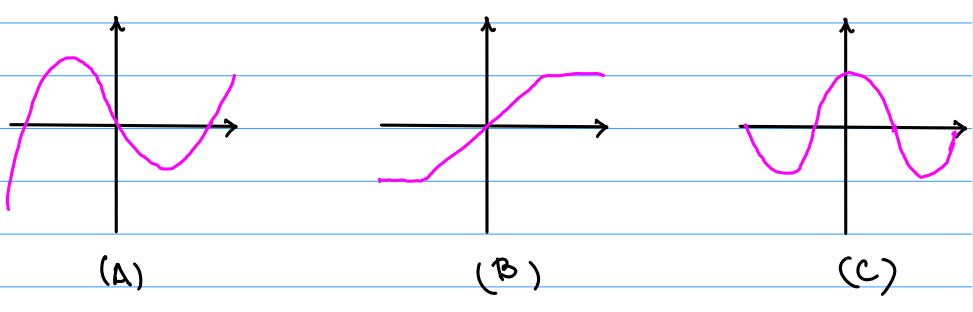
\includegraphics[width=\linewidth]{img/practice_fig1.png}
\vspace{1in}
\end{center}
\begin{center}
\textbf{DERIVATIVES}
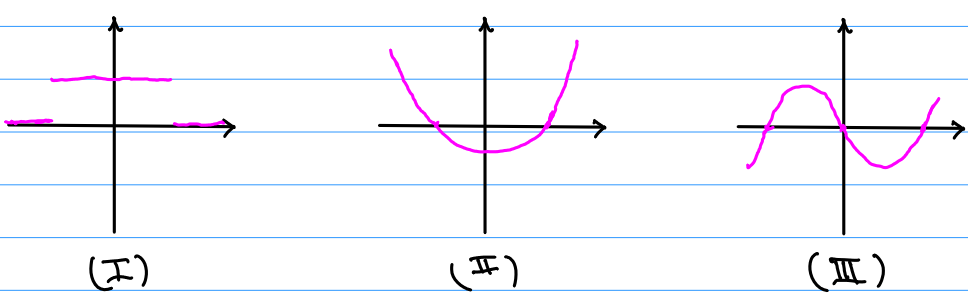
\includegraphics[width=\linewidth]{img/practice_fig2.png}
\end{center}

B-I\\
A-II\\
C-III

\newpage
\question[8]\mbox{}
Consider functions $f(x)$, $g(x)$, and $h(x)$ whose values satisfy
\begin{center}
\begin{tabular}{c|c|c|c|c|c|c|c}
$x$ & 1 & 2 & 3 & 4 & 5 & 6 & 7\\\hline
$f(x)$ & 1 & 1 & 2 & 3 & 5 & 8 & 13\\\hline
$f'(x)$ & 0 & 1 & 3 & 2 & 7 & 9 & 4\\\hline
\end{tabular}\\
\vspace{0.3in}
\begin{tabular}{c|c|c|c|c|c|c|c}
$x$ & 1 & 2 & 3 & 4 & 5 & 6 & 7\\\hline
$g(x)$ & 8 & 6 & 7 & 5 & 3 & 0 & 9\\\hline
$g'(x)$ & 0 & 1 & 0 & 1 & 2 & 3 & 5
\end{tabular}\\
\vspace{0.3in}
\begin{tabular}{c|c|c|c|c|c|c|c}
$x$ & 1 & 2 & 3 & 4 & 5 & 6 & 7\\\hline
$h(x)$ & 2 & 3 & 5 & 7 & 1 & 13 & 17\\\hline
$h'(x)$ & 4 & 3 & 2 & 1 & 2 & 3 & 4
\end{tabular}
\end{center}
Evaluate the following expressions
\begin{enumerate}[(a)]
\item $F(5)$ for $F(x) = 2f(x)+3g(x) + h(x)$ ANS: $2(5)+3(3) + (1) = 20$
\vspace{1in}
\item $F'(5)$ for $F(x) = 2f(x)+3g(x) + h(x)$ ANS: $2(7)+3(2) + (2) = 22$
\vspace{1in}
\item $F(2)$ for $F(x) = h(g(f(4)))$ ANS: $h(g(3))=h(7)=17$
\vspace{1in}
\item $F'(4)$ for $F(x) = x^3 + 3x + h(x)$ ANS: $3(4)^2+3+7=58$
\end{enumerate}


\newpage
\question[10]
Calculate the derivative of each of the following functions.
Carefully show your work, explaining which differentiation rules you are using along the way.
\begin{enumerate}[(a)]
\item $f(x) = x + \cos(x)$
\begin{align*}
f'(x)
 &= (x+\cos(x))'\\
 &= (x)'+(\cos(x))'\quad\text{linearity}\\
 &= 1+(\cos(x))'\quad\text{power law}\\
 &= 1+(-\sin(x))\quad\text{deriv. of trig}\\
\end{align*}
\item $g(t) = \frac{\sqrt{t}+1}{t^2}$
\begin{align*}
g'(t)
 & = \left(\frac{\sqrt{t}+1}{t^2}\right)'\\
 & = \left(\frac{\sqrt{t}}{t^2}+\frac{1}{t^2}\right)'\\
 & = (t^{-3/2}+t^{-2})'\\
 & = (t^{-3/2})'+(t^{-2})'\quad\text{linearity}\\
 & = (-\frac{3}{2}\cdot t^{-3/2-1})+(-2\cdot t^{-2-1})\quad\text{power rule}\\
 & = (-\frac{3}{2}\cdot t^{-5/2})+(-2\cdot t^{-3}) = -\frac{3}{2\sqrt{t^5}} - \frac{2}{t^3}
\end{align*}
\item $h(\theta) = (\theta + \theta^3)^2$
\begin{align*}
h'(x)
 & = ((\theta + \theta^3)^2)'\\
 & = (\theta^2 + 2\theta^4 + \theta^6)'\\
 & = (\theta^2)' + 2(\theta^4)' + (\theta^6)'\quad\text{linearity}\\
 & = (2\theta^{2-1}) + 2(4\theta^{4-1}) + (6\theta^{6-1})\quad\text{power law}\\
 & = 2\theta + 8\theta^3 + 6\theta^5
\end{align*}
\end{enumerate}

\newpage
\question[10]
\begin{enumerate}[(a)]
\item Write down the $\epsilon$,$\delta$-definition of a limit.
We write $\lim_{x\rightarrow a} f(x) = L$ if for all $\epsilon > 0$ there exists $\delta > 0$ such that when $0 < |x-a| < \delta$ we must have $|f(x)-L|<\epsilon$.
\item Let $f(x) = \sqrt{x}$.  Find a value of $$\delta > 0$$ such that if
$$|x-4| < \delta\quad\text{implies}\quad |f(x)-2| < 0.1$$
We need $|x-4| < \delta$ to imply $|\sqrt{x}-2| < 0.1$.
Note that $|\sqrt{x}-2| < 0.1$ means that $\sqrt{x}$ is somewhere within a distance of $0.1$ from $2$, meaning it lies in the interval $(1.9,2.1)$.
This means $x$ should lie within the interval $(1.9^2,2.1^2)$, ie. $(3.61,4.41)$.
The smaller of $4-3.61=0.39$ and $4.41-4$ is $0.39$, so we take $\delta = 0.39$
\end{enumerate}


\newpage
\question[7]
Using only the formal definition of a derivative and any limit laws, calculate the derivative of
$$f(x) = \sqrt{2x+1}.$$
We calculate
\begin{align*}
f'(x)
  &= \lim_{h\rightarrow0}\frac{\sqrt{2(x+h)+1}-\sqrt{2x+1}}{h}\\
  &= \lim_{h\rightarrow0}\frac{\sqrt{2(x+h)+1}-\sqrt{2x+1}}{h}\frac{\sqrt{2(x+h)+1}+\sqrt{2x+1}}{\sqrt{2(x+h)+1}+\sqrt{2x+1}}\\
  &= \lim_{h\rightarrow0}\frac{2(x+h)+1-(2x+1)}{h(\sqrt{2(x+h)+1}+\sqrt{2x+1})}\\
  &= \lim_{h\rightarrow0}\frac{2h}{h(\sqrt{2(x+h)+1}+\sqrt{2x+1})}\\
  &= \lim_{h\rightarrow0}\frac{2}{(\sqrt{2(x+h)+1}+\sqrt{2x+1})}\\
  &= \lim_{h\rightarrow0}\frac{2}{(\sqrt{2(x+0)+1}+\sqrt{2x+1})}\\
  &= \frac{2}{2\sqrt{2x+1}} = \frac{1}{\sqrt{2x+1}}.
\end{align*}

\newpage
\question[7]
Let $a$ and $b$ be constants and consider the function
$$f(x) = \left\lbrace\begin{array}{cc}
x^2 + x & 0\leq x < 1\\
a + bx  & x\geq 1
\end{array}\right.$$
\begin{enumerate}[(a)]
\item For which values of $a$ and $b$ is $f(x)$ continuous at $x=1$?
\vspace{3in}
\item For which values of $a$ and $b$ is $f(x)$ differentiable at $x=1$?
\end{enumerate}

For continuity, we take the left and right limits and find $$1^2 + 1 = a + b(1)$$, so it will be continuous as long as $a+b=2$.
For differentiability, we look at the derivative to the left of $1$, which is $2x+1$, and the derivative to the right, which is $b$.  For these to match up at $1$, we should expect $2(1) + 1 = b$, so $b=3$.  Then since differentiability implies continuity, we should still have $a+b=2$, so we must have $a=-1$.

\end{questions}
\end{document}
